\subsection{Apache Kafka}
\subsubsection{Giới thiệu}
Kafka là hệ thống log message hỗ trợ phân tán, phân vùng và nhân bản; hệ thống thông điệp dạng publish-subcribe. Kafka được thiết kế với những tính chất:
\begin{itemize}
	\item \textit{Persistent messaging}: Hạn chế mất mát thông tin với dữ liệu lớn, độ phức tạp in/out là hằng số (O(1)) kể cả với dữ liệu lớn (TB). Với Kafka thông điệp được lưu trữ trên ổ cứng cũng như được nhân rộng trong cluster để ngăn ngừa việc mất dữ liệu.
	\item \textit{High throughput}: Hỗ trợ vài triệu messages/s đối với những thiết bị phần cứng thông thường
	\item \textit{Distributed}: Message được phân vùng trên những Kafka server khác nhau và việc consume cũng có thể phân tán trên nhóm consumer mà vẫn đảm bảo được tính thứ tự trên mỗi phân vùng.
	\item \textit{Multiple client support}: Tương thích với nhiều client trên các nền tảng khác nhau (java, php, .net, python....)
	\item \textit{Real time}: Consumer ngay lập tức có thể nhận được message tạo bởi producer
\end{itemize}
\begin{figure}[h]
    \centering
    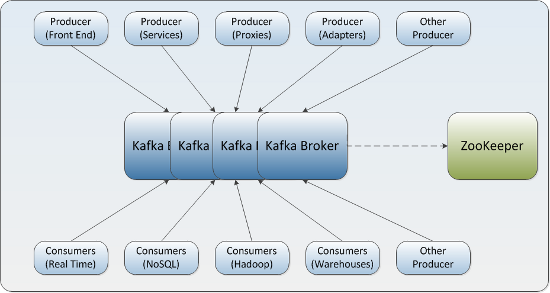
\includegraphics[width=1\textwidth]{kafka-system}
    \caption{Apache Kafka messaging system}
    \label{fig:kafka-system}
\end{figure}
Các thuật ngữ cơ bản:
\begin{itemize}
	\item \textit{Topic}: Kafka lưu trữ message trong các nhóm (categories).
	\item \textit{Producer}: tiến trình đẩy message vào Kafka topic
	\item \textit{Consumer}: tiến trình nhận message từ kafka topic mà nó subscribe
	\item \textit{Broker}: Kafka chạy trên một nhóm các server, mỗi server trong đó gọi là một broker
\end{itemize}
\subsubsection{Topic}

